\chapter{UML diagramy}
	\section{Usecase diagram použitia SCADA systémov}
	\begin{figure}[H]
		\centering
		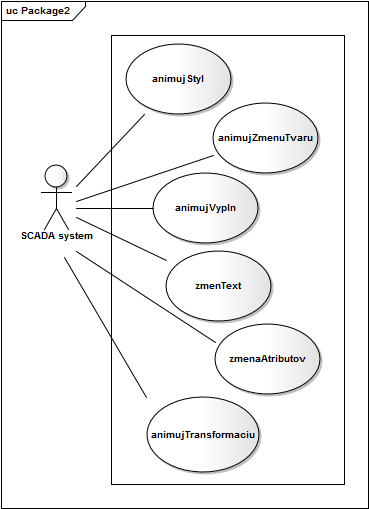
\includegraphics[width=0.50\linewidth]{uml/usecase.png}
		\caption{Usecase diagram použitia SCADA systémov}
		\label{fig:USECASE}
	\end{figure}

	\section{Postup načítania SVG súboru v HTML}
\begin{figure}[H]
	\centering
	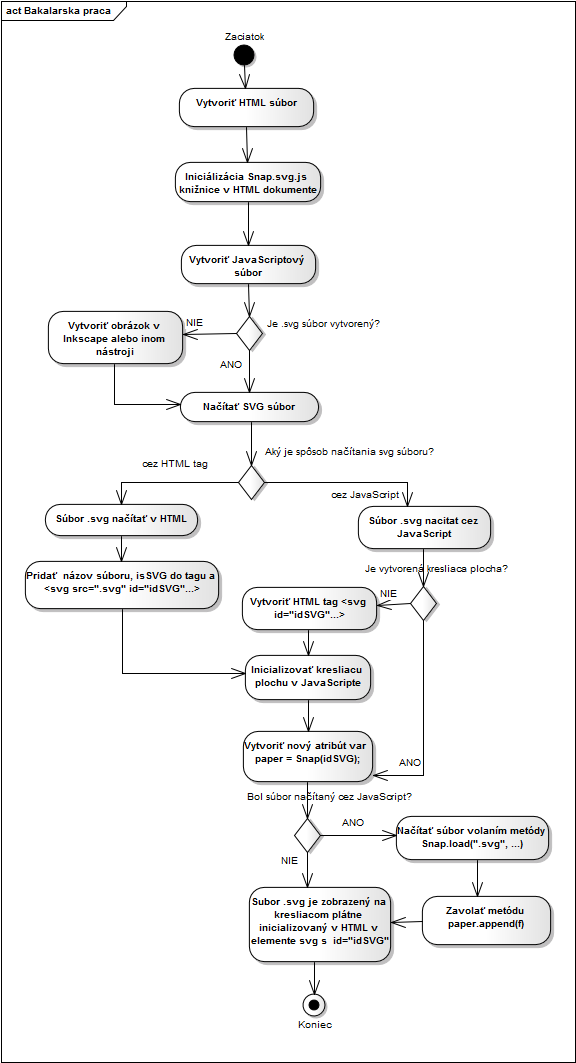
\includegraphics[width=0.6\linewidth]{uml/aktivityInicializacie}
	\caption{Postup načítania SVG súboru v HTML dokumente}
	\label{fig:aktivity1}
\end{figure}

\section{Postup zistenia id elementu}

\begin{figure}[H]
	\centering
	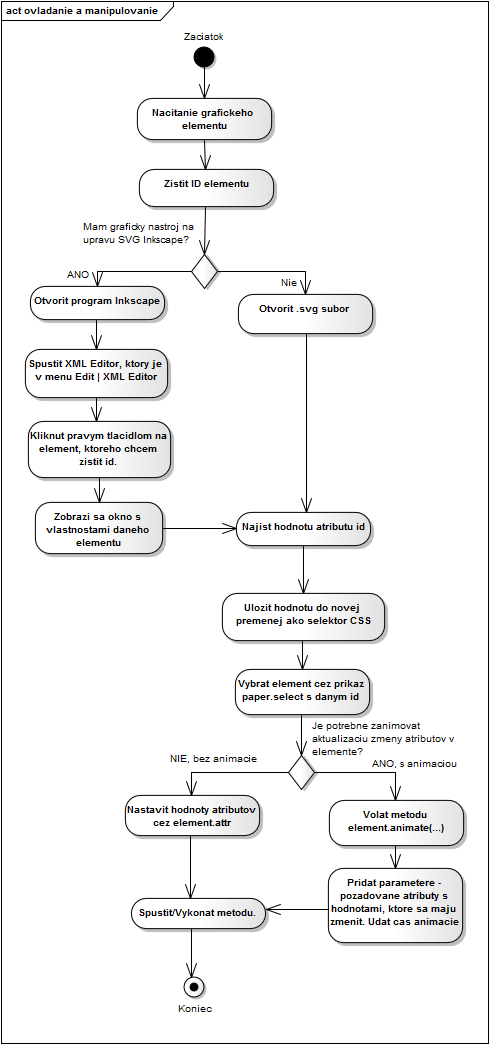
\includegraphics[width=0.6\linewidth]{uml/aktivity2.png}
	\caption{Postup zistenia id elementu a jeho aktualizovanie}
	\label{fig:ovladanie}
\end{figure}







\section{Diagram tried vzorovej sady}
Diagram tried vzorovej sady je na obrázku \ref{fig:classD} . 
\begin{figure}[hp]
	\centering
	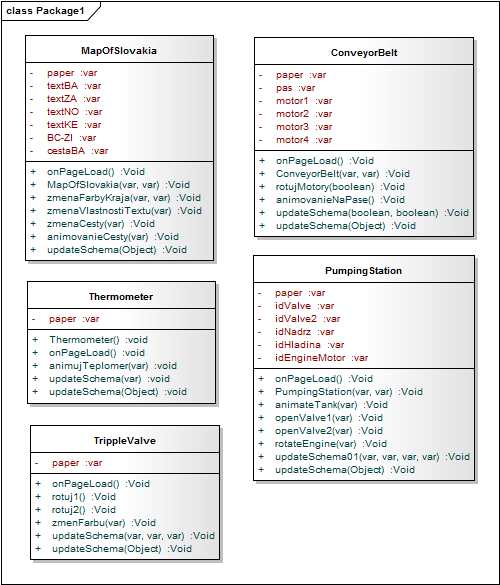
\includegraphics[width=0.9\linewidth]{uml/classDiagramTried}
	\caption{Diagram tried vzorovej sady grafických komponetov}
	\label{fig:classD}
\end{figure}
